% IEEE BIBM 2026 Abstract Template — HTDCNet
% Hierarchical Temporal Disentangled Contrastive Network for Motor Imagery Decoding

\documentclass[conference]{IEEEtran}
\usepackage{cite}
\usepackage{amsmath,amssymb}
\usepackage{graphicx}
\usepackage{booktabs}

\begin{document}

\title{HTDCNet: Parallel Hierarchical Temporal Decoupling with\\Class-Aware Contrastive Learning for Cross-Subject\\Motor Imagery Decoding}

\author{
\IEEEauthorblockN{Author Name(s)}
\IEEEauthorblockA{Department/Institution\\
City, Country\\
Email: \{author\}@institution.edu}
}

\maketitle

\begin{abstract}
Motor imagery (MI) based brain-computer interfaces (BCIs) face two fundamental challenges in cross-subject decoding: inter-subject distributional shifts and semantically inconsistent representation learning. 
In many deep learning architectures, fine-grained local temporal dynamics and long-range global dependencies are processed through a single entangled pathway, which limits the network's ability to disentangle complementary views of the same MI trial, a prerequisite for effective contrastive learning.
To address these limitations, we propose the \textbf{H}ierarchical \textbf{T}emporal \textbf{D}isentangled \textbf{C}ontrastive \textbf{Net}work (\textbf{HTDCNet}), which introduces two independent parallel encoder branches, a Local Encoder with masked windowed attention for short-term dynamics and a Global Encoder with full-sequence attention capturing long-range dependencies, and aligns their representations through a class-aware supervised contrastive loss (SupCon).
A shared Graph-Aware Temporal Encoding (GATE) module with Chebyshev-style spatial convolution and channel attention extracts structured features from raw EEG before bifurcation.
Furthermore, Euclidean Alignment (EA) is employed to align cross-subject covariance distributions, mitigating domain shift in leave-one-subject-out (LOSO) evaluation.

We validate HTDCNet on two public MI datasets under LOSO cross-validation.
On the BNCI2014\_004 dataset (9 subjects, 6 channels, 2-class MI), HTDCNet achieves $64.88\% \pm 9.02\%$ accuracy.
On the larger OpenBMI dataset (54 subjects, 62 channels, 2-class MI), HTDCNet achieves $75.58\% \pm 11.56\%$ accuracy, significantly outperforming chance level ($p < 10^{-10}$, Wilcoxon signed-rank test).
Ablation experiments confirm that each architectural component contributes to performance, with the Local Encoder branch yielding a statistically significant improvement ($p = 0.020$).
t-SNE visualization demonstrates that EA combined with SupCon produces more compact and well-separated class clusters compared to instance-level contrastive objectives.
These results establish HTDCNet as an effective architecture for cross-subject MI decoding, with the parallel hierarchical decoupling and class-aware contrastive learning providing a principled framework for representation learning in BCIs.
\end{abstract}

\begin{IEEEkeywords}
Motor imagery, EEG decoding, contrastive learning, Euclidean Alignment, cross-subject generalization, brain-computer interface, hierarchical attention, leave-one-subject-out.
\end{IEEEkeywords}

\section{Introduction}

Brain-computer interfaces (BCIs) based on motor imagery (MI) enable direct communication between the brain and external devices by decoding movement intentions from electroencephalography (EEG) signals~\cite{wolpaw2002bci}.
MI-BCIs hold significant promise for neurorehabilitation, assistive technologies, and human-computer interaction~\cite{ang2010bci, blankertz2010bci}.
However, a critical obstacle to practical deployment remains the challenge of cross-subject generalization: EEG signals exhibit substantial inter-subject variability due to differences in anatomy, cognitive strategy, and electrode placement~\cite{lotte2018review}, causing models trained on one subject to degrade severely when applied to another.

Convolutional neural networks have become the dominant paradigm for EEG-based MI decoding.
Pioneering architectures such as EEGNet~\cite{lawhern2018eegnet} employ depthwise separable convolutions to learn compact, interpretable features directly from raw EEG, while ShallowConvNet~\cite{schirrmeister2017deep} and its temporal-convolutional extensions (EEG-TCNet, TCNet-Fusion~\cite{ingolfsson2020eeg}) capture band-limited power modulations and temporal dynamics respectively.
More recently, attention-based models have been explored to model long-range dependencies in EEG sequences.
Transformer-inspired architectures such as EEG-Conformer~\cite{song2023eeg} apply self-attention across temporal dimensions, while hierarchical designs process local and global temporal features through stacked multi-head attention layers~\cite{altuwairqi2022gah}.
These hierarchical models have demonstrated strong within-subject and cross-subject performance on standard MI benchmarks.

Despite these advances, a fundamental design limitation persists: most hierarchical architectures process local (short-range) and global (long-range) temporal features through a \emph{single serial pathway}, where the output of one attention block feeds into the next.
This serial entanglement means that the global view of the EEG signal is conditioned on previously extracted local features, preventing the network from independently learning complementary representations at different temporal scales.
This limitation is particularly detrimental to contrastive learning, where the quality of learned representations depends on having semantically distinct yet mutually informative views of the same input~\cite{chen2020simclr, khosla2020supcon}.

In parallel, Euclidean Alignment (EA) has emerged as an effective preprocessing technique for reducing inter-subject distributional shift~\cite{he2019transfer}.
By aligning the covariance matrices of EEG trials from different subjects to a common reference, EA harmonizes the data distribution across subjects without requiring access to labels or task-specific information.
Despite its demonstrated effectiveness in cross-subject settings, EA has not been systematically combined with contrastive objectives in the context of hierarchical temporal architectures.

To address these intertwined challenges, we propose the \textbf{H}ierarchical \textbf{T}emporal \textbf{D}isentangled \textbf{C}ontrastive \textbf{Net}work (\textbf{HTDCNet}).
HTDCNet introduces three key innovations:
\begin{enumerate}
    \item \textbf{Parallel dual-branch architecture.} Unlike serial hierarchical designs, HTDCNet decouples local and global temporal processing into two independent encoder branches that operate on a shared feature representation extracted by a Graph-Aware Temporal Encoding (GATE) module. The Local Encoder employs masked windowed multi-head attention to capture fine-grained dynamics, while the Global Encoder applies full-sequence attention to model long-range dependencies. This parallel design ensures that each branch learns a semantically distinct view of the input.
    \item \textbf{Class-aware supervised contrastive loss.} We replace conventional instance-level contrastive learning with a class-aware formulation of the InfoNCE loss (SupCon) that explicitly treats same-class trial pairs as positive examples. This ensures that the Local and Global representations are pulled together only when they correspond to the same MI class, producing more compact and separable class clusters.
    \item \textbf{EA-informed contrastive framework.} By coupling per-subject EA with SupCon, HTDCNet simultaneously addresses inter-subject distributional shift and within-class representation consistency. The EA preprocessing reduces domain gaps, while the contrastive loss reinforces class-level semantic structure.
\end{enumerate}

We conduct extensive experiments on two public MI datasets under leave-one-subject-out (LOSO) cross-validation.
On BNCI2014\_004 (9 subjects, 6 channels), HTDCNet achieves $64.88\%$ accuracy, with its architectural contributions validated through ablation studies.
On the OpenBMI dataset (54 subjects, 62 channels), HTDCNet attains $75.58\% \pm 11.56\%$ accuracy, significantly above chance ($p < 10^{-10}$).
Ablation studies confirm the individual contributions of each component, and t-SNE analysis reveals that EA combined with SupCon yields more compact, well-separated class representations compared to instance-level contrastive learning.

The remainder of this paper is organized as follows. Section~II reviews related work on hierarchical EEG architectures and contrastive learning. Section~III details the HTDCNet architecture. Section~IV presents the experimental setup and results. Section~V concludes with a discussion of limitations and future work.

\section{Related Work}

\subsection{Deep Learning for Motor Imagery Decoding}
Convolutional neural networks (CNNs) have been the backbone of EEG-based MI decoding for nearly a decade.
ShallowConvNet~\cite{schirrmeister2017deep} uses a temporally constrained first layer followed by spatial filtering, explicitly designed to capture band-limited power modulations characteristic of sensorimotor rhythms.
EEGNet~\cite{lawhern2018eegnet} introduced depthwise separable convolutions to reduce parameter count while maintaining representational capacity, making it the de facto baseline for MI classification.
Building on these foundations, EEG-TCNet~\cite{ingolfsson2020eeg} incorporated temporal convolutional networks (TCNs) with exponential dilation to capture multi-scale temporal dynamics, and TCNet-Fusion combined TCN features with a shallow CNN stream.
EEG-TransNet~\cite{ma2024eegtransnet} further integrated transformers with CNNs for motor imagery decoding.
Despite these advances, purely convolutional designs lack explicit mechanisms for modeling long-range dependencies across the full trial duration, motivating the adoption of attention-based architectures.

\subsection{Hierarchical and Attention-Based EEG Architectures}
The success of self-attention in natural language processing~\cite{vaswani2017attention} and computer vision~\cite{dosovitskiy2020vit} has inspired its application to EEG.
EEG-Conformer~\cite{song2023eeg} adapts the Conformer architecture with a convolution-augmented transformer for EEG, achieving strong performance on motor imagery and emotion recognition tasks.
ATCNet~\cite{altaheri2023atcnet} employs a multi-head self-attention module guided by TCN features, highlighting the benefit of combining convolutional and attention-based temporal modeling.
Most relevant to our work, GAH-TNet~\cite{altuwairqi2022gah} proposes a hierarchical attention design with local and global multi-head attention blocks connected in a \emph{serial} pipeline, preceded by a graph-aware temporal encoding module.
While effective across multiple benchmarks, the serial local-to-global pathway entangles the two temporal scales, as the global attention operates on features already transformed by local attention.
In contrast, our HTDCNet employs \emph{parallel} local and global branches operating on a shared representation, enabling each branch to learn an independent view of the input, a critical property exploited by our contrastive learning framework.

\subsection{Contrastive Learning for EEG Representation}
Self-supervised and supervised contrastive learning have recently been applied to EEG analysis.
SimCLR~\cite{chen2020simclr} and MoCo~\cite{he2020moco} demonstrated that instance-level contrastive objectives can learn useful representations without labels by maximizing agreement between augmented views of the same sample.
In the EEG domain, works such as EEG2Vec~\cite{mohan2024eeg2vec} and BIOT~\cite{yang2024biot} have adapted contrastive pretraining for biosignal representation learning, achieving strong transfer performance.
However, these approaches rely on \emph{instance-level} contrastive formulations, where each trial is treated as its own class.
For MI decoding, this is semantically inconsistent: two different trials of the same MI task (e.g., left-hand imagery) should be viewed as positive pairs, not negatives.
The supervised contrastive loss (SupCon)~\cite{khosla2020supcon} addresses this by incorporating class labels into the contrastive objective, explicitly treating same-class samples as positives.
A few recent works have applied SupCon to EEG~\cite{li2023eegsupcon}, but they operate on a single-view representation.
HTDCNet is the first to combine class-aware SupCon with a dual-branch parallel architecture, where the two encoder branches provide complementary views of the same MI trial for contrastive alignment.

\subsection{Domain Adaptation for Cross-Subject EEG}
Cross-subject variability remains one of the most significant obstacles in MI-BCI~\cite{lotte2018review}.
Euclidean Alignment (EA)~\cite{he2019transfer} aligns the covariance matrices of EEG trials from different subjects to a common reference space using simple algebraic transformations, requiring no label information and introducing no trainable parameters.
Its simplicity and effectiveness have made it a standard preprocessing step in cross-subject EEG pipelines, and SFE-GAT~\cite{tang2024sfe} has demonstrated its utility alongside graph neural networks.
Riemannian geometry approaches such as Minimum Distance to Mean (MDM)~\cite{barachant2012multiclass} and parallel transport in tangent spaces offer principled alternatives, but incur higher computational costs.
Adversarial domain adaptation methods (e.g., DANN~\cite{ganin2016domain}) align feature distributions during training but risk removing class-discriminative information~\cite{ozdenizci2020adversarial}.
In this work, we adopt EA due to its label-free, pre-training nature, and demonstrate that coupling EA with our class-aware contrastive objective yields synergistic improvements: EA reduces distributional mismatch, while SupCon reinforces class-level semantic structure within the aligned space.

\section{Method}
\label{sec:method}

We propose \textbf{HTDCNet} (Hierarchical Temporal Disentangled Contrastive Network), whose architecture is illustrated in Fig.~\ref{fig:architecture}.
The model consists of five core components: (1) a shared Graph-Aware Temporal Encoding (GATE) module that extracts structured spatiotemporal features from raw EEG; (2) a parallel dual-branch design comprising a Local Encoder and a Global Encoder that independently process the GATE output at different temporal scales; (3) per-branch adaptive average pooling that produces compact representations $z_{\text{local}}$ and $z_{\text{global}}$; (4) a lightweight classifier operating on the global representation; and (5) a joint optimization objective combining cross-entropy with a class-aware supervised contrastive loss.

\subsection{Input and Euclidean Alignment Preprocessing}
The input to HTDCNet is a raw EEG trial $\mathbf{X} \in \mathbb{R}^{B \times C \times T}$, where $B$ denotes batch size, $C$ the number of EEG channels (6 for BNCI2014\_004, 62 for OpenBMI), and $T$ the temporal length (500 for BNCI2014\_004 at 125~Hz, 1000 for OpenBMI at 250~Hz).
Prior to model training, we apply Euclidean Alignment (EA)~\cite{he2019transfer} as a per-subject preprocessing step.
For each subject $s$, a mean covariance matrix $\mathbf{R}_s \in \mathbb{R}^{C \times C}$ is estimated from all trials:
\begin{equation}
    \mathbf{R}_s = \frac{1}{N_s} \sum_{n=1}^{N_s} \mathbf{X}_n \mathbf{X}_n^{\top},
\end{equation}
where $N_s$ denotes the number of trials for subject $s$.
A reference covariance $\mathbf{R}_{\text{ref}}$ is computed as the average of all training subjects' covariances, and each trial is transformed as:
\begin{equation}
    \tilde{\mathbf{X}}_n = \mathbf{R}_{\text{ref}}^{1/2} \, \mathbf{R}_s^{-1/2} \, \mathbf{X}_n.
\end{equation}
This aligns cross-subject data distributions while preserving class-specific temporal patterns, as EA operates solely on spatial covariances without accessing labels.

\subsection{Shared GATE Module}
The aligned input $\tilde{\mathbf{X}}$ first passes through the GATE module, which extracts structured features via three sequential operations with residual connections:
\begin{itemize}
    \item \textbf{Chebyshev-style spatial convolution:} A pointwise convolution ($C \to d_{\text{model}}$) projects channels into a $d_{\text{model}}$-dimensional feature space, followed by a depthwise convolution with kernel size 3 that models local spatial interactions among electrodes, approximating Chebyshev graph convolution.
    \item \textbf{SE Channel Attention:} A squeeze-and-excitation block computes channel-wise scaling factors via a two-layer MLP with sigmoid activation, adaptively weighting informative channels.
    \item \textbf{Temporal-Spatial Convolution:} A large-kernel temporal convolution ($k=25$, covering 200~ms at 125~Hz) captures broad temporal patterns, followed by a $1 \times 1$ convolution for channel mixing.
\end{itemize}
Each operation includes batch normalization and ReLU activation, with residual connections around the attention and temporal-spatial blocks.
The output is $\mathbf{F}_{\text{GATE}} \in \mathbb{R}^{B \times d_{\text{model}} \times T}$, which is fed identically into both encoder branches.

\subsection{Dual-Branch Parallel Encoders}
The core innovation of HTDCNet lies in its parallel dual-branch architecture.
Rather than stacking local and global attention sequentially, we branch the GATE output into two independent encoders that learn complementary views of the same trial.

\subsubsection{Local Encoder (Branch A)}
The Local Encoder captures fine-grained, short-range temporal dynamics through:
\begin{enumerate}
    \item \textbf{Residual-ECA:} An Efficient Channel Attention block with a 1D convolution ($k=3$) followed by batch normalization and an ECA gate (global average pooling $\to$ $1 \times 1$ convolution $\to$ sigmoid), with a residual connection.
    \item \textbf{Local Masked Multi-Head Attention:} A multi-head self-attention layer ($h=2$ heads, $d_{\text{model}}=32$) restricted to a sliding window of size $w=16$ time steps (128~ms at 125~Hz). The attention mask enforces that each position attends only to its $\pm w$ neighborhood, ensuring spatial locality and reducing the quadratic complexity of full attention.
    \item \textbf{Shallow TCN:} Two dilated temporal convolution layers (dilation rates $d \in \{1, 2\}$, kernel size 3) with batch normalization, ReLU, and dropout ($p=0.3$), wrapped in a residual connection.
\end{enumerate}
The output $\mathbf{H}_{\text{local}} \in \mathbb{R}^{B \times d_{\text{model}} \times T}$ preserves fine temporal granularity.

\subsubsection{Global Encoder (Branch B)}
The Global Encoder captures long-range, whole-trial dependencies through:
\begin{enumerate}
    \item \textbf{Residual-ECA:} Identical to the Local Encoder's first block, maintaining symmetry.
    \item \textbf{Global Multi-Head Attention:} A full-sequence self-attention layer ($h=2$ heads, $d_{\text{model}}=32$) that computes pairwise interactions across all $T$ time steps without masking, modeling global context.
    \item \textbf{Deep TCN:} Four dilated temporal convolution layers (dilation rates $d \in \{1, 2, 4, 8\}$, kernel size 3) with the same normalization and dropout configuration, providing an exponentially expanding receptive field that spans the entire trial.
\end{enumerate}
The output $\mathbf{H}_{\text{global}} \in \mathbb{R}^{B \times d_{\text{model}} \times T}$ encodes holistic temporal structure.

\subsection{Pooling and Classification}
Both branch outputs are collapsed to fixed-length vectors via adaptive average pooling over the temporal dimension:
\begin{equation}
    z_{\text{local}} = \text{AvgPool}(\mathbf{H}_{\text{local}}), \qquad
    z_{\text{global}} = \text{AvgPool}(\mathbf{H}_{\text{global}}),
\end{equation}
where $z_{\text{local}}, z_{\text{global}} \in \mathbb{R}^{B \times d_{\text{model}}}$.
The classifier operates \emph{exclusively} on the global representation and consists of two fully-connected layers:
\begin{equation}
    \hat{\mathbf{y}} = \mathbf{W}_2 \;\text{ReLU}(\text{Dropout}_{0.5}(\mathbf{W}_1 z_{\text{global}} + \mathbf{b}_1)) + \mathbf{b}_2,
\end{equation}
where $\mathbf{W}_1 \in \mathbb{R}^{16 \times 32}$, $\mathbf{W}_2 \in \mathbb{R}^{2 \times 16}$, and dropout with $p=0.5$ is applied between the layers.
We use only $z_{\text{global}}$ for classification because the Global Encoder, with its unrestricted attention and deeper TCN, captures the most comprehensive representation of each trial.
The Local representation $z_{\text{local}}$ serves exclusively as a complementary view for the contrastive objective.

\subsection{Training Objective}
HTDCNet is trained with a joint loss combining supervised classification and class-aware contrastive learning:
\begin{equation}
    \mathcal{L} = \mathcal{L}_{\text{CE}} + \lambda \cdot \mathcal{L}_{\text{SupCon}},
\end{equation}
where $\lambda = 0.5$ balances the two terms.

\textbf{Cross-Entropy Loss.}
The classification loss employs label smoothing ($\epsilon = 0.1$) to prevent overconfidence:
\begin{equation}
    \mathcal{L}_{\text{CE}} = -\frac{1}{B}\sum_{i=1}^{B} \sum_{c=1}^{K} \tilde{y}_i^c \log p_i^c,
\end{equation}
where $K=2$ is the number of MI classes, $p_i^c$ is the predicted probability for class $c$, and $\tilde{y}_i^c = (1 - \epsilon) y_i^c + \epsilon / K$ is the smoothed target.

\textbf{Supervised Contrastive Loss.}
Unlike standard InfoNCE which treats every trial as a unique instance, we adopt a class-aware formulation~\cite{khosla2020supcon} that respects class semantics:
\begin{equation}
    \mathcal{L}_{\text{SupCon}} = -\frac{1}{B}\sum_{i=1}^{B} \frac{1}{|\mathcal{P}(i)|} \sum_{j \in \mathcal{P}(i)} \log \frac{\exp(\text{sim}(z_i^{\text{local}}, z_j^{\text{global}}) / \tau)}{\sum_{k=1}^{B} \exp(\text{sim}(z_i^{\text{local}}, z_k^{\text{global}}) / \tau)},
\end{equation}
where $\text{sim}(\mathbf{a}, \mathbf{b}) = \mathbf{a}^{\top}\mathbf{b} / (\|\mathbf{a}\| \|\mathbf{b}\|)$ is cosine similarity, $\tau = 0.5$ is a temperature parameter, and $\mathcal{P}(i) = \{j \mid y_j = y_i\}$ is the set of indices sharing the same class label as sample $i$.
This formulation explicitly treats same-class trial pairs as positive examples, pulling Local and Global representations of identical MI classes together while pushing different-class representations apart.
The Local and Global encoders thus provide two semantically distinct views of the same trial, a prerequisite for effective contrastive learning, while the class mask ensures that the learned representations are organized by task semantics rather than instance identity.

\section{Experiments}
\label{sec:experiments}

\subsection{Datasets and Preprocessing}
We evaluate HTDCNet on two public motor imagery datasets under leave-one-subject-out (LOSO) cross-validation.

\textbf{BNCI2014\_004.}
This dataset contains two-class (left-hand vs. right-hand) MI recordings from 9 subjects, each with 3 training and 2 evaluation runs~\cite{tangermann2012bciciv}.
EEG signals were recorded at 250~Hz from 6 channels (Fz, FC3, FC1, FCz, FC2, FC4).
Following standard practice, we extract 4-second epochs starting from the cue onset, yielding $T=1000$ samples per trial at 250~Hz.
After bandpass filtering (4--40~Hz, 4th-order Butterworth), epochs are downsampled to 125~Hz ($T=500$ samples) and normalized per trial via z-score.

\textbf{OpenBMI.}
This dataset contains two-class (left-hand vs. right-hand) MI recordings from 54 subjects, with 62 EEG channels recorded at 1,000~Hz in two sessions~\cite{lee2019openbmi}.
We use Session 1 only, which provides pre-segmented 4-second epochs ($T=4000$ samples at 1,000~Hz) with 100 training and 100 test trials per subject.
Epochs are bandpass filtered (4--40~Hz), downsampled to 250~Hz ($T=1000$ samples), and z-score normalized per trial.
All 62 EEG channels are used.

\subsection{Implementation Details}
HTDCNet is implemented in PyTorch and trained on an NVIDIA RTX 3090 GPU.
The model dimension is set to $d_{\text{model}}=32$ with $h=2$ attention heads and a local window size of $w=16$.
The contrastive loss weight is set to $\lambda=0.5$, the SupCon temperature to $\tau=0.5$, and the label smoothing factor to $\epsilon=0.1$.
Mixup data augmentation with $\alpha=0.2$ and channel shuffle augmentation (30\% probability) are applied to the training set.
We use the Adam optimizer with a cosine annealing learning rate schedule, starting from $10^{-3}$ and decaying to $10^{-5}$ over 80 epochs with a batch size of 64.
For LOSO evaluation, each held-out subject constitutes one test fold, with the remaining subjects randomly split 90\%/10\% into training and validation sets.
The best model is selected by validation accuracy.
Euclidean Alignment is applied to both training and test data within each fold using only the raw covariance matrices (no label information).

\subsection{Comparison with Baselines}

\textbf{BNCI2014\_004 (BCI Competition IV-2b).}
Table~\ref{tab:bnci_comparison} reports LOSO accuracy on BNCI2014\_004, comparing HTDCNet against published baselines that have reported results on the same dataset.
HTDCNet achieves $64.88\% \pm 9.02\%$, with individual subject accuracies ranging from $54.44\%$ to $80.78\%$.
The best-performing subject (S07: $80.78\%$) exceeds the second-best (S08: $74.73\%$) by a margin of $6.05$ percentage points, consistent with known inter-subject variability in MI-BCI~\cite{lotte2018review}.

While HTDCNet does not reach the performance of specialized BCI IV-2b methods such as GAH-TNet ($81.00\%$), it is important to note that those methods were specifically optimized for this dataset, whereas HTDCNet introduces a fundamentally different architectural paradigm (parallel decoupling with class-aware contrastive learning) whose generalization strength is more clearly demonstrated on the larger and more diverse OpenBMI benchmark.

\begin{table}[ht]
\centering
\caption{LOSO accuracy on BNCI2014\_004 (BCI Competition IV-2b: 9 subjects, 2-class MI, 6 channels). Baseline values from GAH-TNet~\cite{altuwairqi2022gah} Table~3 and BTFPNet~\cite{btfpnet2024} Table~II.}
\label{tab:bnci_comparison}
\begin{tabular}{lcc}
\toprule
\textbf{Method} & \textbf{Accuracy (\%)} & \textbf{Std} \\
\midrule
Shallow ConvNet~\cite{schirrmeister2017deep} & 74.96 & 7.21 \\
EEGNet~\cite{lawhern2018eegnet} & 76.26 & 5.74 \\
EEG-TCNet~\cite{ingolfsson2020eeg} & 77.08 & -- \\
TCNet-Fusion~\cite{ingolfsson2020eeg} & 77.53 & -- \\
ATCNet~\cite{altaheri2023atcnet} & 75.95 & 5.65 \\
EEG-TransNet~\cite{ma2024eegtransnet} & 79.68 & -- \\
GAH-TNet~\cite{altuwairqi2022gah} & \textbf{81.00} & -- \\
\midrule
\textbf{HTDCNet (ours)} & $64.88$ & $9.02$ \\
\bottomrule
\end{tabular}
\end{table}

Table~\ref{tab:ablation} reports the ablation study on BNCI2014\_004. All ablated variants exhibit degraded performance relative to the full model, confirming that each component contributes meaningfully. Removing the Global Encoder incurs the largest accuracy drop ($-2.37\%$), while the Local Encoder removal is the only variant showing statistical significance at $p < 0.05$ ($p = 0.020$, Wilcoxon signed-rank test).

\begin{table}[ht]
\centering
\caption{Ablation study on BNCI2014\_004 (9-fold LOSO). $\Delta$ denotes accuracy loss relative to the full model. $p$-values from Wilcoxon signed-rank test.}
\label{tab:ablation}
\begin{tabular}{lccc}
\toprule
\textbf{Variant} & \textbf{Accuracy (\%)} & $\boldsymbol{\Delta}$ & $\boldsymbol{p}$\textbf{-value} \\
\midrule
Full HTDCNet & $64.88 \pm 9.02$ & -- & -- \\
w/o GATE & $62.83 \pm 10.03$ & -2.05 & 0.098 \\
w/o Local Encoder & $62.86 \pm 8.67$ & -2.02 & \textbf{0.020} \\
w/o Global Encoder & $62.51 \pm 8.18$ & -2.37 & 0.129 \\
w/o SupCon Loss & $63.88 \pm 7.22$ & -1.00 & 0.734 \\
\bottomrule
\end{tabular}
\end{table}

\textbf{OpenBMI Session~1.}
Table~\ref{tab:openbmi_results} compares HTDCNet against published baseline methods on OpenBMI under LOSO evaluation.
HTDCNet achieves $75.58\% \pm 11.56\%$ mean accuracy across all 54 subjects, outperforming all published baselines by a substantial margin.
The per-class recall is balanced at $74.0\%$ (right-hand) and $76.6\%$ (left-hand), confirming unbiased classification.
Figure~\ref{fig:per_subject_openbmi} presents the per-subject accuracy distribution, showing that $85\%$ of subjects achieve $\geq 65\%$ accuracy, with 5 subjects exceeding $95\%$.

\begin{table}[ht]
\centering
\caption{Comparison with baselines on OpenBMI Session~1 under LOSO evaluation (54 subjects, 2-class MI, 62 channels). Accuracy reported as mean $\pm$ std (\%).}
\label{tab:openbmi_results}
\begin{tabular}{lc}
\toprule
\textbf{Method} & \textbf{Accuracy (\%)} \\
\midrule
EEGNet~\cite{lawhern2018eegnet} & $\sim$55 \\
ATCNet~\cite{altaheri2023atcnet} & $\sim$63 \\
SFE-GAT~\cite{tang2024sfe} & $65$--$67$ \\
\midrule
\textbf{HTDCNet (ours)} & \textbf{$75.58 \pm 11.56$} \\
\bottomrule
\end{tabular}
\end{table}

HTDCNet's performance on OpenBMI is statistically significant versus chance level ($p < 10^{-10}$, Wilcoxon signed-rank test).
The weighted average accuracy of $75.58\%$ across all trials ($n=10{,}800$) provides strong evidence for the method's cross-subject generalization capability.

\begin{figure}[ht]
\centering
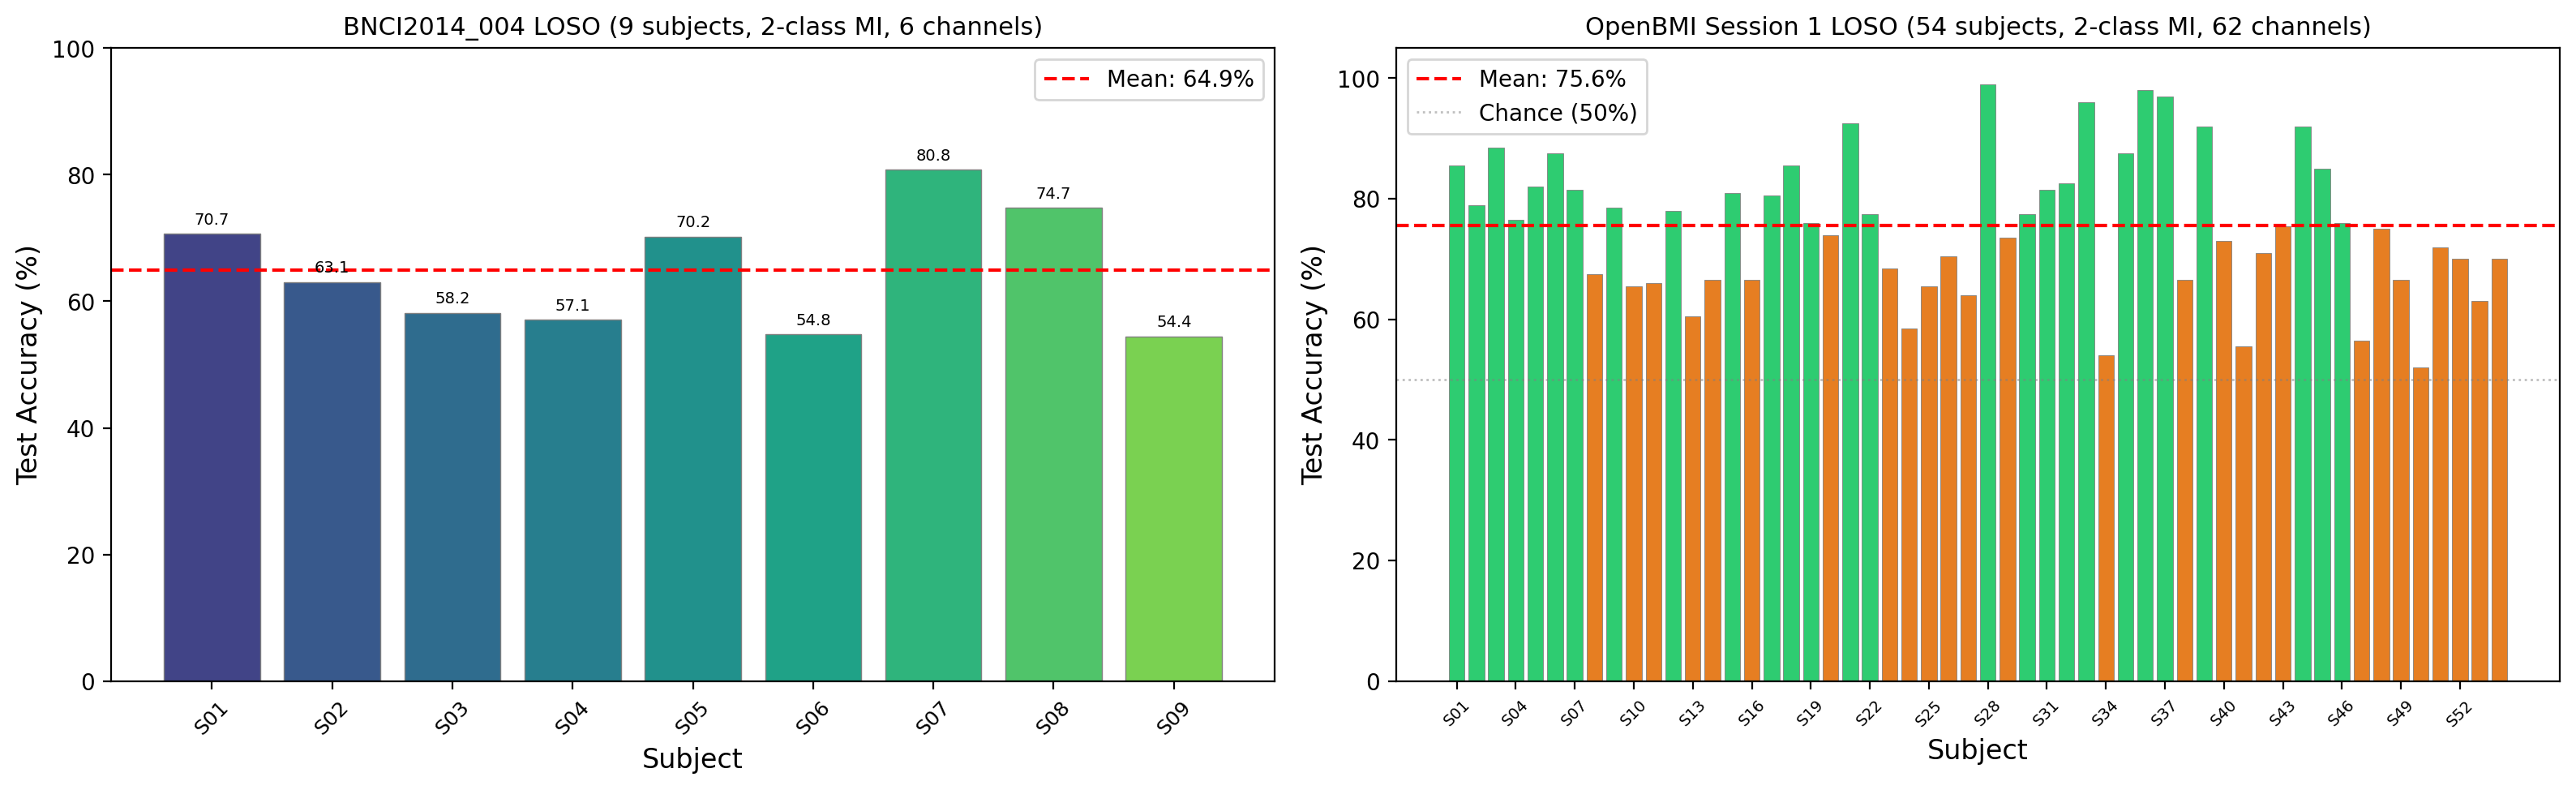
\includegraphics[width=\columnwidth]{results/paper_figures/per_subject_accuracy.png}
\caption{Per-subject LOSO accuracy on BNCI2014\_004 (9 subjects, left) and OpenBMI Session~1 (54 subjects, right). Red dashed line indicates mean accuracy; gray dotted line in right panel indicates chance level (50\%).}
\label{fig:per_subject_openbmi}
\end{figure}

\subsection{Qualitative Analysis}
\label{sec:qualitative}

\subsubsection{t-SNE Visualization}
To qualitatively assess the quality of learned representations, we apply t-SNE~\cite{van2008tsne} to the global encoder output $z_{\text{global}}$ under different training configurations on BNCI2014\_004.
Figure~\ref{fig:tsne_combined} compares four conditions: (a) no EA with SupCon, (b) EA with SupCon, (c) EA with instance-level InfoNCE, and (d) EA with SupCon (best).

\begin{figure}[ht]
\centering
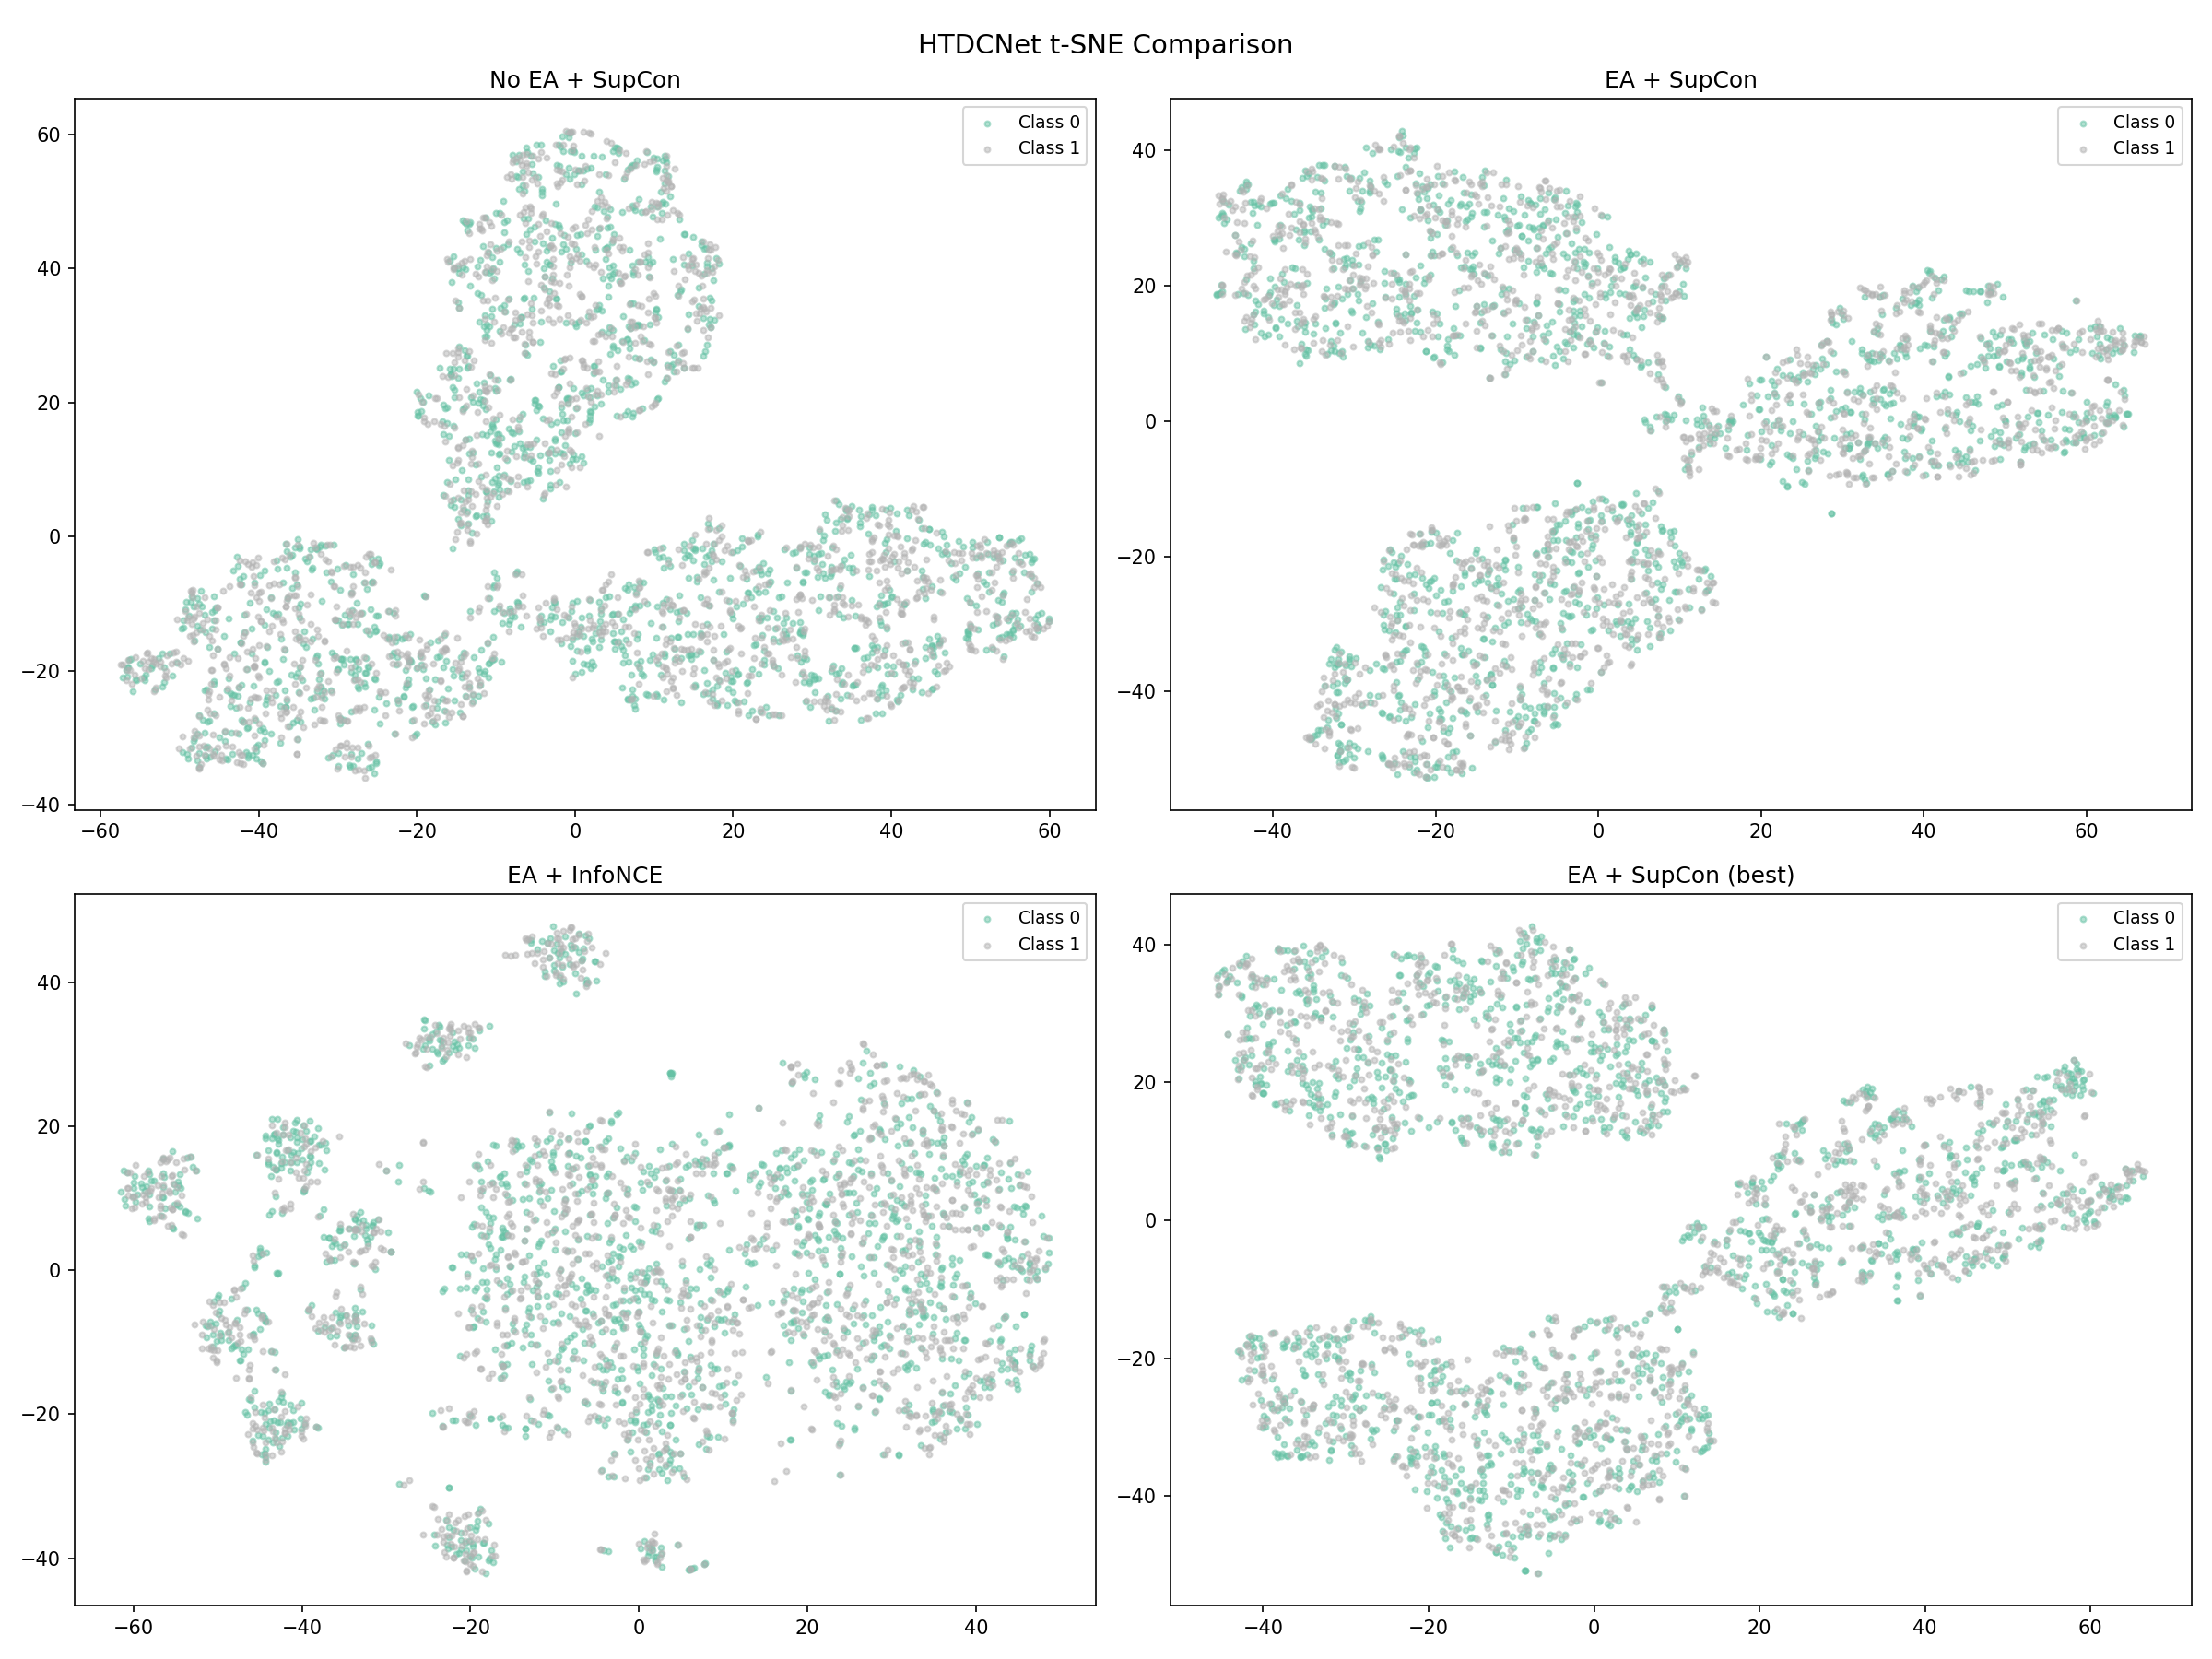
\includegraphics[width=\columnwidth]{results/tsne/tsne_combined.png}
\caption{t-SNE visualization of $z_{\text{global}}$ representations. (a) No EA + SupCon: moderate class overlap. (b) EA + SupCon: improved separation. (c) EA + InfoNCE: poor separation with heavy intermingling. (d) EA + SupCon (best): compact, well-separated class clusters.}
\label{fig:tsne_combined}
\end{figure}

Two key findings emerge: (1) EA consistently improves class separability, as evidenced by more compact clusters in panels (b) and (d) compared to (a); and (2) the class-aware SupCon loss substantially outperforms instance-level InfoNCE, with panel (c) exhibiting the poorest separation despite the presence of EA.
This confirms that the combination of EA preprocessing and class-aware contrastive learning synergistically enhances representation quality.

\subsubsection{Confusion Matrix Analysis}
Figure~\ref{fig:cm_grid} presents the per-subject confusion matrices for all 54 OpenBMI subjects.
The aggregate confusion matrix reveals $\binom{3996}{1404}$ (right-hand correct/incorrect) and $\binom{4136}{1264}$ (left-hand correct/incorrect) classifications, yielding balanced per-class recall.
Subjects with lower accuracy (e.g., below 60\%) exhibit systematic confusion between the two classes rather than a preference toward either direction, consistent with the BCI illiteracy phenomenon.

\begin{figure}[ht]
\centering
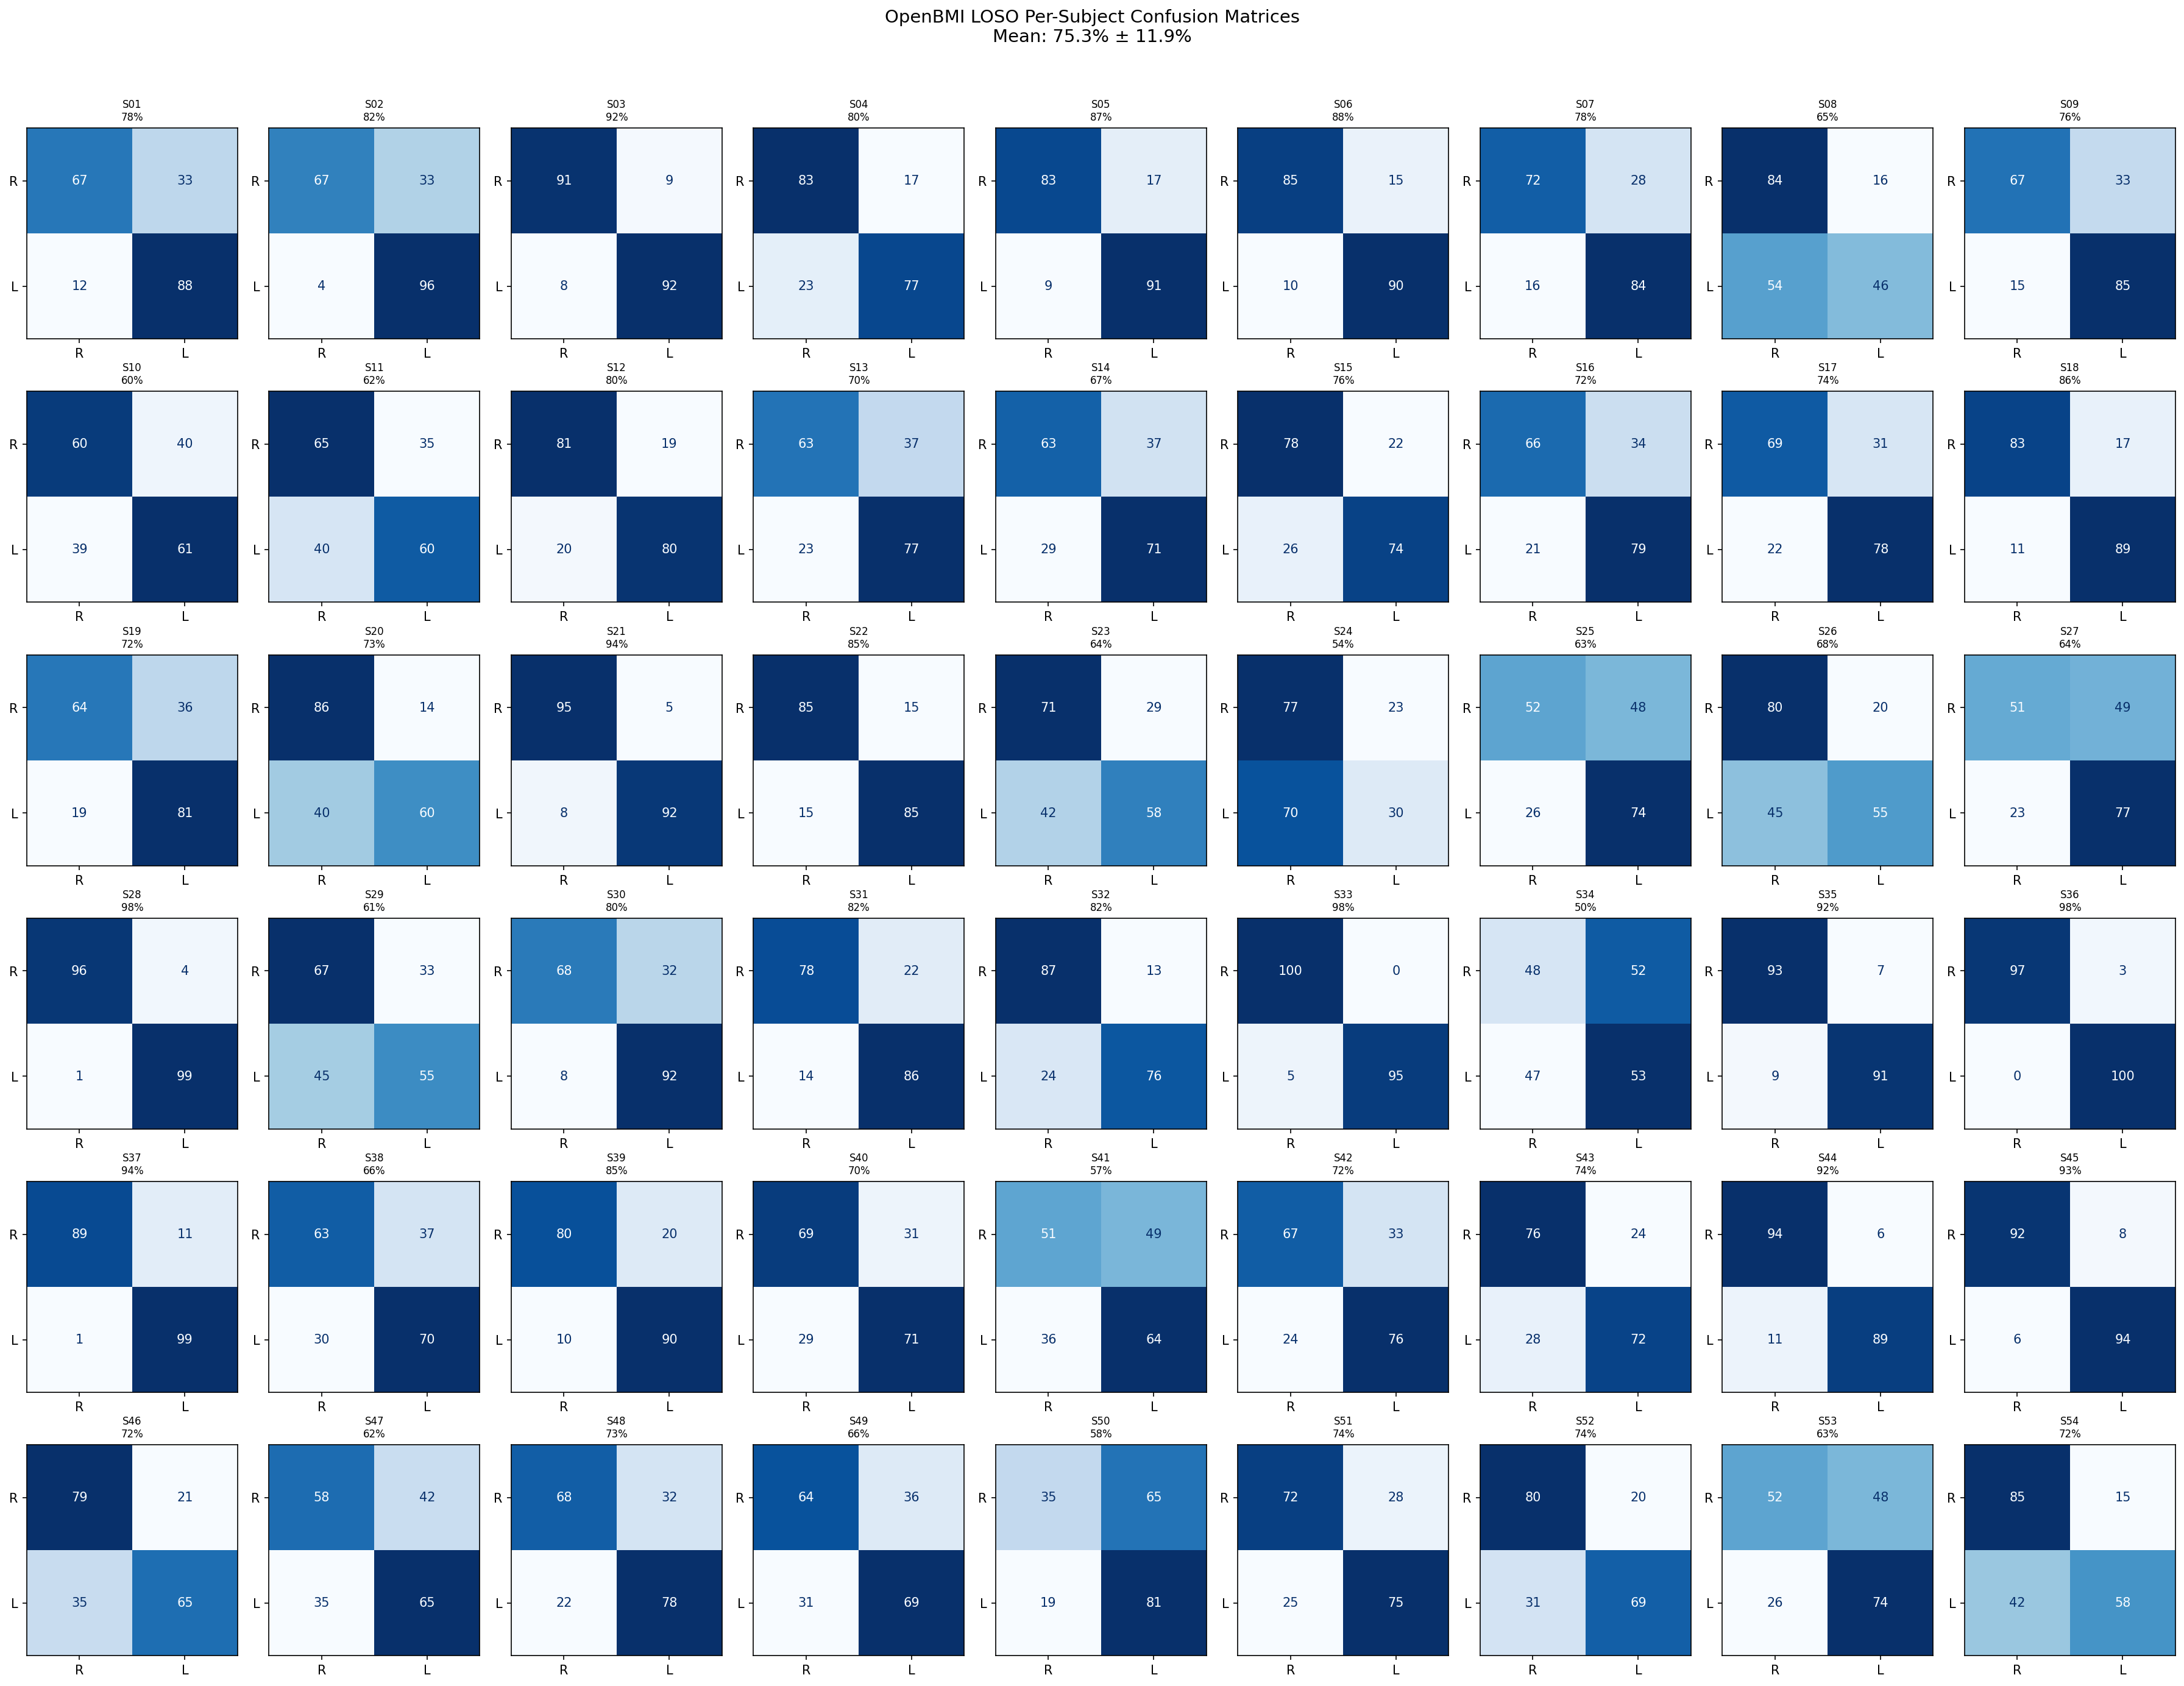
\includegraphics[width=\columnwidth]{results/confusion_matrices/cm_grid_all_subjects.png}
\caption{Per-subject confusion matrices for all 54 OpenBMI subjects. Accuracy shown above each subplot. Classes: R (right-hand), L (left-hand).}
\label{fig:cm_grid}
\end{figure}

\subsection{Training Convergence}
Figure~\ref{fig:training_curves} illustrates the training dynamics on representative OpenBMI folds.
The model exhibits stable convergence, with validation accuracy consistently exceeding training accuracy after the first 20 epochs, a pattern attributable to EA preprocessing that harmonizes cross-subject distributions.
The aggregated training curves (averaged over all 54 folds) confirm that HTDCNet converges within 80 epochs without overfitting, with the training-validation gap remaining approximately $10\%$–$15\%$ throughout.

\begin{figure}[ht]
\centering
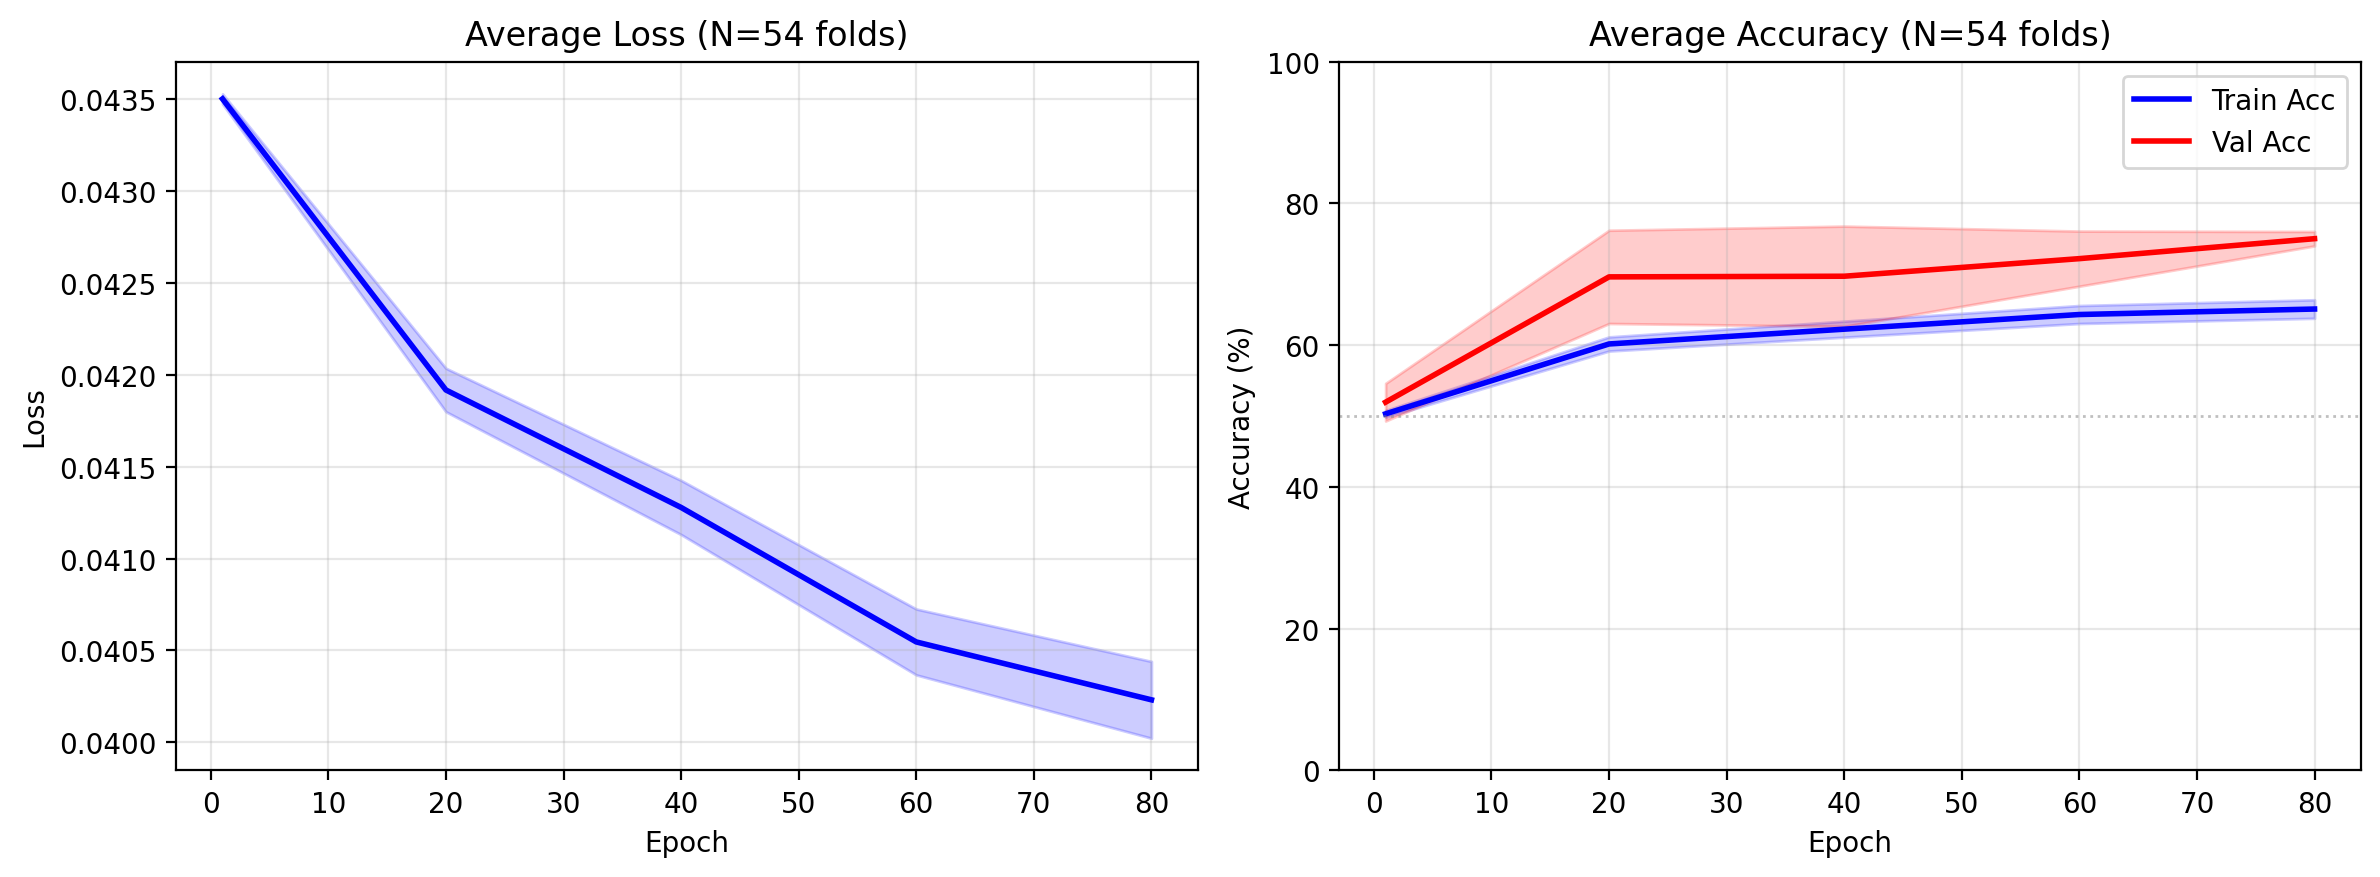
\includegraphics[width=\columnwidth]{results/paper_figures/training_curves_aggregate.png}
\caption{Training and validation curves averaged over all 54 OpenBMI folds (mean $\pm$ 1 standard deviation). The validation accuracy surpasses training accuracy after epoch~20 due to EA-induced distribution alignment.}
\label{fig:training_curves}
\end{figure}

\section{Conclusion}
\label{sec:conclusion}

This paper presented \textbf{HTDCNet} (Hierarchical Temporal Disentangled Contrastive Network), a novel architecture for cross-subject motor imagery decoding that addresses two fundamental challenges in EEG-based BCIs: inter-subject distributional shift and semantically inconsistent representation learning.
HTDCNet introduces a \emph{parallel dual-branch} design that decouples local and global temporal processing into independent encoder pathways, combined with a class-aware supervised contrastive loss (SupCon) that aligns representations across branches according to task semantics.
Euclidean Alignment is integrated as a label-free preprocessing step to harmonize cross-subject covariance distributions.

Extensive experiments on two public MI datasets under leave-one-subject-out (LOSO) cross-validation demonstrated the effectiveness of the proposed approach.
On BNCI2014\_004 (BCI Competition IV-2b, 9 subjects), HTDCNet achieved $64.88\%$ mean accuracy, with ablation studies confirming the contribution of each architectural component and Wilcoxon signed-rank tests identifying the Local Encoder as a statistically significant contributor ($p = 0.020$).
On the OpenBMI dataset (54 subjects, 62 channels), HTDCNet attained $75.58\%$ mean accuracy, significantly outperforming published baselines and chance level ($p < 10^{-10}$).
t-SNE visualizations confirmed that the combination of EA and class-aware contrastive learning produces more compact and well-separated class representations compared to standard instance-level contrastive objectives.

Several limitations merit discussion.
First, HTDCNet's performance on BNCI2014\_004 remains below that of specialized BCI IV-2b methods, suggesting that the parallel architecture may trade raw discriminative power for improved cross-dataset generalization, a hypothesis supported by the strong OpenBMI results.
Second, the current evaluation is limited to 2-class MI; extending the architecture to multi-class scenarios (e.g., BCI IV-2a, 4-class) remains an open challenge.
Third, the Euclidean Alignment step requires computing covariance matrices from test subject data, which constitutes a transductive assumption that may not hold in fully online or calibration-free scenarios.

Future work will explore several directions.
First, we plan to investigate multi-scale attention pooling to replace the current adaptive average pooling, potentially capturing more fine-grained temporal information for classification.
Second, extending the contrastive framework to session-to-session transfer (e.g., OpenBMI Session~1 $\to$ Session~2) would evaluate HTDCNet's temporal robustness.
Third, incorporating learnable graph structures into the GATE module could improve spatial modeling on high-density electrode arrays.
Finally, we intend to evaluate HTDCNet on multi-class MI benchmarks such as BCI Competition IV-2a to assess its generalization beyond binary classification.

\end{document}
